\documentclass{standalone}
% %%%%%%%%%%%%%%%%%%%%%%%%%%%%%%%%%%%%%%%%%%%%%%%%%%%
% %%%%%%%%%%%%%%%%%%%%%%%%%%%%%%%%%%%%%%%%%%%%%%%%%%%

\usepackage[default,semibold]{../../../../../../Latex-workspace/beamer-templates-v3/sourcesanspro/tex/sourcesanspro}
\usepackage{fontspec}
\setmainfont{SourceSansPro}

% les packages pour la gestion des couleurs
\usepackage{color}
%\usepackage{xcolor}
\usepackage[x11names]{xcolor}

\usepackage{tikz}
\usetikzlibrary{shapes}
\usetikzlibrary{decorations.pathreplacing}
\usetikzlibrary{arrows,automata,positioning}
\usetikzlibrary{shapes.symbols}
\usetikzlibrary{arrows.meta}
\usetikzlibrary{shapes,snakes}


% %%%%%%%%%%%%%%%%%%%%%%%%%%%%%%%%%%%%%%%%%%%%%%%%%%%
% %%%%%%%%%%%%%%%%%%%%%%%%%%%%%%%%%%%%%%%%%%%%%%%%%%%
% The main document 
\begin{document}     
% %%%%%%%%%%%%%%%%%%%%%%%%%%%%%%%%%%%%%%%%%%%%%%%%%%%
% %%%%%%%%%%%%%%%%%%%%%%%%%%%%%%%%%%%%%%%%%%%%%%%%%%%
% %%%%%%%%%%%%%%%%%%%%%%%%%%%%%%%%%%%%%%%%%%%%%%%%%%%
% %%%%%%%%%%%%%%%%%%%%%%%%%%%%%%%%%%%%%%%%%%%%%%%%%%%

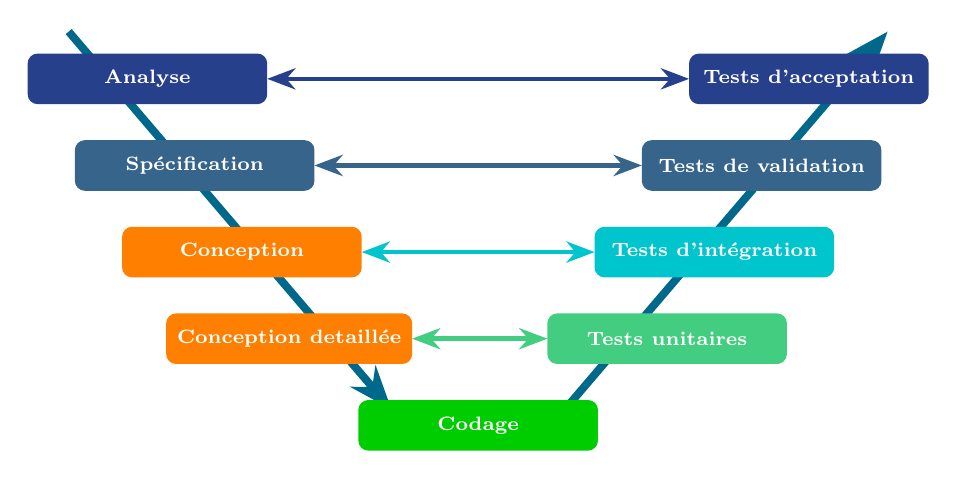
\begin{tikzpicture}
    \tikzstyle{dev-step}=[rectangle, draw,  rounded corners=3pt, minimum width=3.0cm,  minimum height=0.6cm, very thick, font=\scriptsize\bfseries]
    \tikzstyle{fleche}=[-Stealth, ultra thick]

    \draw[fleche, line width=1mm, color=DeepSkyBlue4] (-5.2, 5.0) -- (-1.1,0.2);
    \draw[fleche, line width=1mm, color=DeepSkyBlue4] (1.1,0.2) -- (5.2, 5.0);

    \node[dev-step, color=Green3, fill=Green3] (codage) at (0,0) {\textcolor{white}{Codage}};

    \node[dev-step, color=orange, fill=orange] (conception-detaillee) at (-2.4,1.1) {\textcolor{white}{Conception detaillée}};
    \node[dev-step, color=SeaGreen3, fill=SeaGreen3] (tests-unitaires) at (2.4,1.1) {\textcolor{white}{Tests unitaires}};
    \draw[<->, >= Stealth, ultra thick, color=SeaGreen3] (conception-detaillee) -- (tests-unitaires);

    \node[dev-step, color=orange, fill=orange] (conception) at (-3,2.2) {\textcolor{white}{Conception}};
    \node[dev-step, color=Turquoise3, fill=Turquoise3] (tests-integration) at (3,2.2) {\textcolor{white}{Tests d'intégration}};
    \draw[<->, >= Stealth, ultra thick, color=Turquoise3] (conception) -- (tests-integration);

    \node[dev-step, color=SteelBlue4, fill=SteelBlue4] (specification) at (-3.6,3.3) {\textcolor{white}{Spécification}};
    \node[dev-step, color=SteelBlue4, fill=SteelBlue4] (tests-validation) at (3.6,3.3) {\textcolor{white}{Tests de validation}};
    \draw[<->, >= Stealth, ultra thick, color=SteelBlue4] (specification) -- (tests-validation);

    \node[dev-step, color=RoyalBlue4, fill=RoyalBlue4] (analyse) at (-4.2,4.4) {\textcolor{white}{Analyse}};
    \node[dev-step, color=RoyalBlue4, fill=RoyalBlue4] (tests-acceptation) at (4.2,4.4) {\textcolor{white}{Tests d'acceptation}};
    \draw[<->, >= Stealth, ultra thick, color=RoyalBlue4] (analyse) -- (tests-acceptation);
\end{tikzpicture}

% %%%%%%%%%%%%%%%%%%%%%%%%%%%%%%%%%%%%%%%%%%%%%%%%%%%
% %%%%%%%%%%%%%%%%%%%%%%%%%%%%%%%%%%%%%%%%%%%%%%%%%%% 
\end{document}
% %%%%%%%%%%%%%%%%%%%%%%%%%%%%%%%%%%%%%%%%%%%%%%%%%%%
% %%%%%%%%%%%%%%%%%%%%%%%%%%%%%%%%%%%%%%%%%%%%%%%%%%%